\begin{figure}[h]
\centering
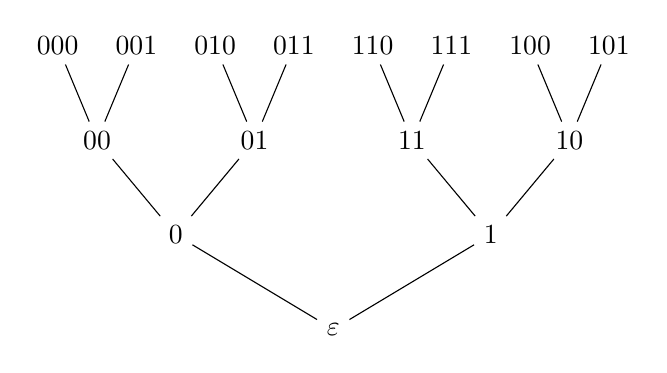
\begin{tikzpicture}[level distance=1.2cm,
  level 1/.style={sibling distance=4cm},
  level 2/.style={sibling distance=2cm},
  level 3/.style={sibling distance=1cm},
  grow=up
  ]
  \node {$\varepsilon$}
    child {node {1}
      child {node {10}
        child {node {101}}
        child {node {100}}
      }
      child {node {11}
        child {node {111}}
        child {node {110}}
      }
    }
    child {node {0}
      child {node {01}
        child {node {011}}
        child {node {010}}
      }
      child {node {00}
        child {node {001}}
        child {node {000}}
      }
    };
\end{tikzpicture}
\caption{درخت دودویی $T^*$ تا سطح $l=3$}
\end{figure}